%-------------------------------------------------------------------------------
%                                PREAMBLE
%-------------------------------------------------------------------------------
\documentclass[usenames,dvipsnames,svgnames,10pt,aspectratio=169]{beamer}
%
\usefonttheme{professionalfonts}
% This theme uses TIKZ: compile twice with PDFLaTeX or LuaLaTeX.
%
%  Options:
%  - [clean]:    clean slides, i.e. logos and footbar are removed
%  - [kth]:      footbar style inspierd to the official KTH template
%  - [nicewave]: a different style of wave is used (not approved by FLOW)
%
\usetheme[clean]{flow}

\usepackage{tikz}
\usepackage{pgfplots}
\usepgfplotslibrary{polar}

\usepackage{hyperref,graphicx,lmodern}
\usepackage[utf8]{inputenc}
\usepackage{media9}
\usepackage{xcolor}
\usepackage{stmaryrd}
\usepackage{nicefrac}
\usepackage{multimedia}
\usepackage{multicol}
\usepackage{upgreek}
\usepackage[]{bm}
\usepackage[]{url}
\usepackage[]{animate}
\usepackage{amsmath}

\graphicspath{{imgs/}}

%\setbeamertemplate{blocks}[rounded][shadow=true]

\setbeamercolor{background canvas}{bg=black}
\setbeamercolor{frametitle}{fg=white}
\setbeamercolor{normal text}{fg=white}


%-------------------------------------------------------------------------------
%                                TITLE PAGE
%-------------------------------------------------------------------------------
\title[Nonlinear physics] % Short title used in footline
{
	Nonlinear physics, dynamical \\
	systems and chaos theory
}

\author[J.-Ch.~Loiseau] % Presenting author in short form used in footline
{
	\underline{Jean-Christophe Loiseau}
}
% - Give the names in the same order as the appear in the paper.
% - Underline the presenting author.

\institute[unused]
{
	\url{jean-christophe.loiseau@ensam.eu} \\
	Laboratoire DynFluid \\
	Arts et M\'etiers, France.
}
% Keep it simple, no one is interested in your street address.

% University logo(s)
\logot{
\includegraphics[width=.128\paperwidth]{DynFluid_logo}}  % Top logo
\logob{
\includegraphics[width=0.128\paperwidth]{ENSAM_logo}} % Bottom logo
% \logoc[{\includegraphics[width=.128\paperwidth]{limsi}}]{\includegraphics[width=.128\paperwidth]{limsi}} % Corner logo
%
% Cover image: \cvrimg{x position}{y position}{cover image}
\cvrimg{.77}{.8}{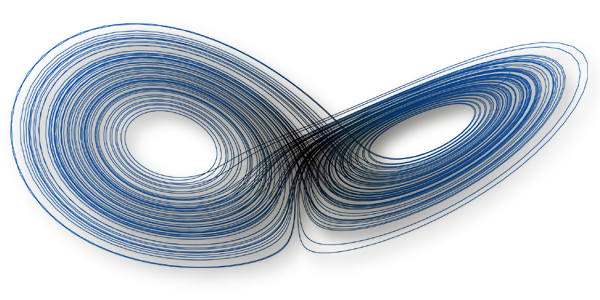
\includegraphics[width=.4\paperwidth]{cover.png}}

\date[unused]{Physique non-lin\'eaire -- 2019-2020}

\begin{document}

\titleframe	% Print the title as the first slide

%-------------------------------------------------------------------------------
%                           PRESENTATION SLIDES
%-------------------------------------------------------------------------------

\begin{frame}[t, c]{Basic information}{Organization}
	\begin{minipage}{.68\textwidth}
		\begin{itemize}
			\item Lectures: Tuesdays and Thurdays, from 3:30pm to 5:30pm.

			\bigskip

			\item Evaluation divided into two parts:
			\begin{itemize}
				\item[\( \hookrightarrow \)] A two-hour long written exam late February.
				\item[\( \hookrightarrow \)] A homework project.
			\end{itemize}
		\end{itemize}
	\end{minipage}%
	\hfill
	\begin{minipage}{.28\textwidth}
		\centering
		
\includegraphics[width=\textwidth]{Gears}
	\end{minipage}

	\vspace{1cm}
\end{frame}

\begin{frame}[t, c]{Basic information}{Homework project}
	\begin{minipage}{.28\textwidth}
		\centering
		
\includegraphics[height=.15\textheight]{python_logo}

		\bigskip

		
\includegraphics[height=.15\textheight]{julia_logo}
	\end{minipage}%
	\hfill
	\begin{minipage}{.68\textwidth}
		\begin{itemize}
			\item Ideally in \alert{\textbf{Python 3}} or \alert{\textbf{Julia}}.
			\begin{itemize}
				\item[\( \hookrightarrow \)] Open-source programming languages for scientific computing.
			\end{itemize}

			\bigskip

			\item You can install both of them from scratch or using \alert{\textbf{Anaconda}}.
			\begin{itemize}
				\item[\( \hookrightarrow \)] Available for Windows, Mac OS and Linux.
			\end{itemize}

		\end{itemize}
	\end{minipage}

	\vspace{1cm}
\end{frame}

\begin{frame}[t, c]{Basic information}{Useful references (in French)}
	\begin{minipage}{.58\textwidth}
		\begin{block}{\centering \textbf{General knowledge}}
			\begin{itemize}
				\item I.\ Stewart. \emph{Dieu joue-t'il au dés?} Flammarion (2004).

				\medskip

				\item J.\ Gleick. \emph{La théorie du chaos.} Flammarion (2008).

				\medskip

				\item I.\ Prigogine. \emph{Les lois du chaos.} Flammarion (2008).
			\end{itemize}
		\end{block}%
		\vfill
		\begin{block}{\centering \textbf{Textbooks}}
			\begin{itemize}
				\item P.\ Bergé \emph{et al.} \emph{L'ordre dans le chaos.} Hermann (1998).

				\medskip

				\item P.\ Manneville. \emph{Instabilités, chaos et turbulence.} Ed.\ Ecole Polytechnique (2004).
			\end{itemize}
		\end{block}
	\end{minipage}%
	\hfill
	\begin{minipage}{.38\textwidth}
		\centering

		
\includegraphics[width=\textwidth]{references}
	\end{minipage}

	\vspace{1cm}
\end{frame}

\begin{frame}[t, c]{Basic information}{Useful references (in English)}
  \begin{minipage}{.58\textwidth}
    \begin{block}{\centering \textbf{Textbooks}}
      \begin{itemize}
        \item P.\ Manneville. \emph{Instabilities, chaos and turbulence.} Ed.\ Ecole Polytechnique (2004).

          \medskip

        \item S. Strogatz. \emph{Nonlinear dynamics and chaos.} 2\textsuperscript{nd} edition, Avalon Publishing (2016).
      \end{itemize}
    \end{block}%
    \vfill
    \begin{block}{\centering \textbf{Online videos}}
      \begin{itemize}
      \item Steve Bruton : \url{https://www.youtube.com/c/Eigensteve/videos}

        \medskip

      \item Prof Gristh Math : \url{https://www.youtube.com/channel/UC5N5pRddyicAX1QJyJjIIdg}
      \end{itemize}
    \end{block}


  \end{minipage}%
  \hfill
  \begin{minipage}{.38\textwidth}
		\centering
		
\includegraphics[width=\textwidth]{references}
  \end{minipage}

  \vspace{1cm}
\end{frame}

\begin{frame}[t, c]{}{}
  \begin{block}{\centering \textbf{What is dynamical systems theory ?}}

    \bigskip

    \centering
    It is the mathematics of behaviour and the classification of how systems evolve over time.
  \end{block}
\end{frame}

%\begin{frame}[t, c]{Some examples}{Celestial Mechanics}
\begin{frame}[t, c]{}{}
  \begin{minipage}{.58\textwidth}
    \centering
    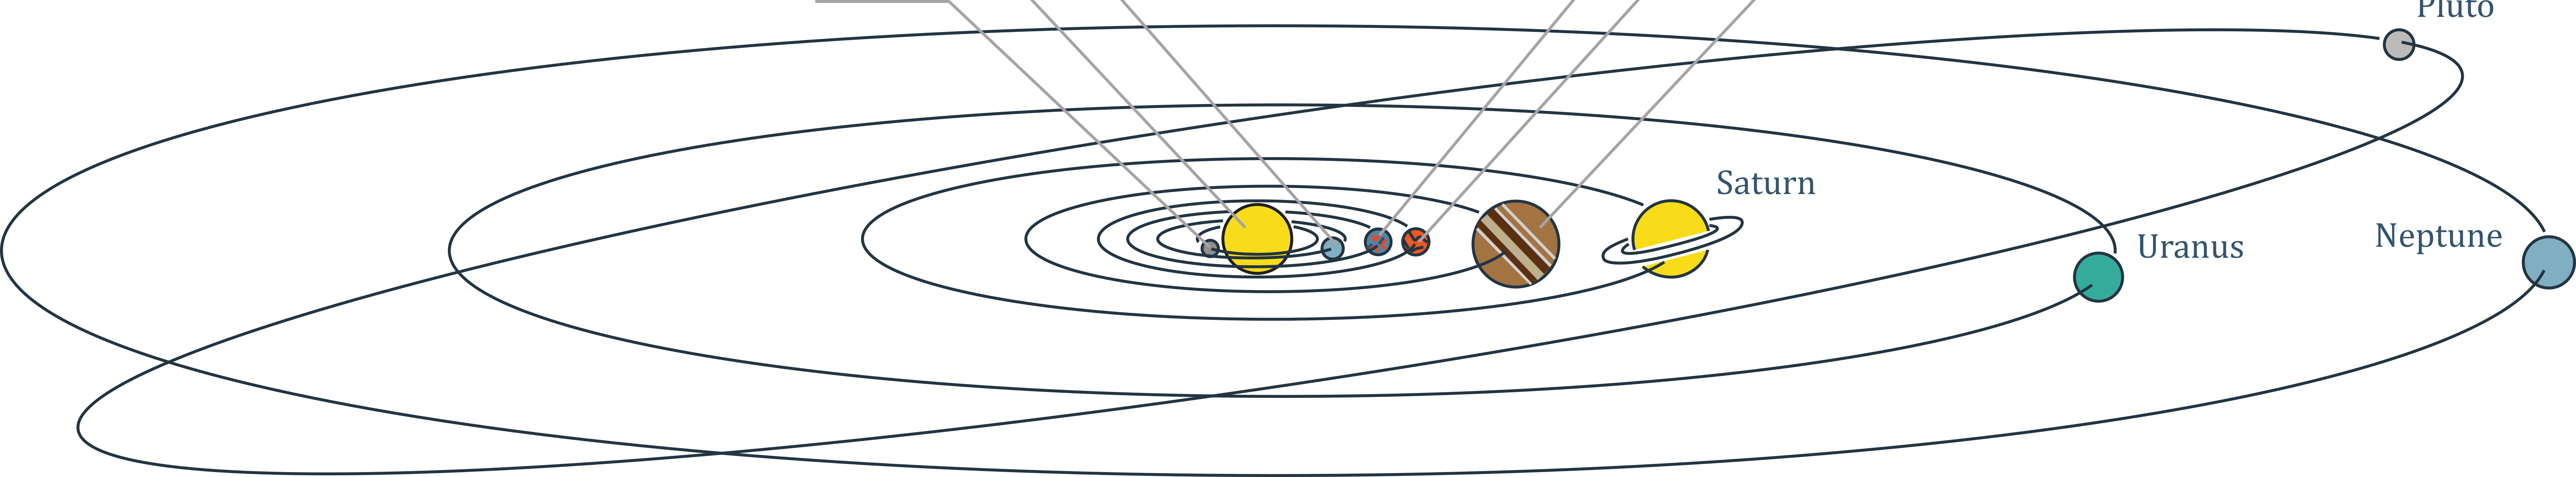
\includegraphics[width=\textwidth]{solar_system}
  \end{minipage}%
  \hfill
  \begin{minipage}{.38\textwidth}
    \centering
    \textbf{Newton's law of gravitation}
    %
    \[
    \ddot{\bm{x}}_j = \sum_{i \neq j}^n \dfrac{G M_i}{\| \bm{x}_i - \bm{x}_j \|^3} \left( \bm{x}_i - \bm{x}_j \right)
    \]
  \end{minipage}

  \vspace{-1cm}
\end{frame}

%\begin{frame}[t, c]{Some examples}{Mechanical Engineering}
\begin{frame}[t, c]{}{}
	\begin{minipage}{.28\textwidth}
		\centering
		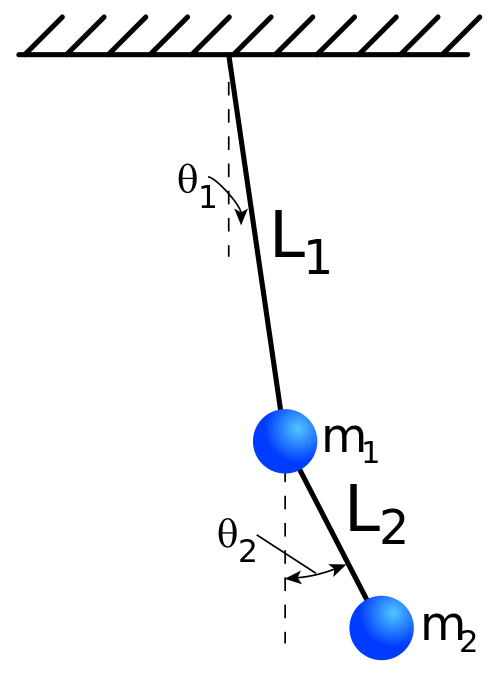
\includegraphics[width=.9\textwidth]{double_pendulum_geometry}
	\end{minipage}%
	\hfill
	\begin{minipage}{.68\textwidth}
    \begin{overprint}
      \onslide<1>
      \centering
      \textbf{Lagrangian Mechanics}
      %
      \[
      \begin{aligned}
        \mathcal{L}(\theta_1, \theta_2, \dot{\theta}_1, \dot{\theta}_2) & = \text{Kinetic Energy} - \text{Potential Energy} \\
        & \dfrac{\mathrm{d}}{\mathrm{dt}} \left( \dfrac{\partial \mathcal{L}}{\partial \dot{\theta}_i} \right) - \dfrac{\partial \mathcal{L}}{\partial \theta_i}  = 0
      \end{aligned}
      \]

      \onslide<2>
      \centering
      \textbf{Hamiltonian Mechanics}
      %
      \[
      \begin{aligned}
        \mathcal{H}(p_1, p_2, q_1, q_2) & = \text{Kinetic Energy} + \text{Potential Energy} \\
        \dfrac{\mathrm{d}p_i}{\mathrm{d}t} & = -\dfrac{\partial \mathcal{H}}{\partial q_i}, \quad \dfrac{\mathrm{d}q_i}{\mathrm{d}t} = \dfrac{\partial \mathcal{H}}{\partial p_i}
      \end{aligned}
      \]
    \end{overprint}
	\end{minipage}

	\vspace{-1cm}  
\end{frame}

%\begin{frame}[t, c]{Some examples}{Mechanical Engineering}
\begin{frame}[t, c]{}{}
	\begin{minipage}{.48\textwidth}
		\begin{itemize}
			\item Simple mechanical sytem exhibiting nonetheless complex dynamics.

			\bigskip

			\item Evolutions of similar initial conditions diverge exponentially fast.

			\bigskip

			\item Limited prediction horizon despite its deterministic equations of motion.
		\end{itemize}
	\end{minipage}%
	\hfill
	\begin{minipage}{.48\textwidth}
		\vspace{-0.25cm}
		\begin{center}
			\movie[width=\textwidth, autostart, loop]{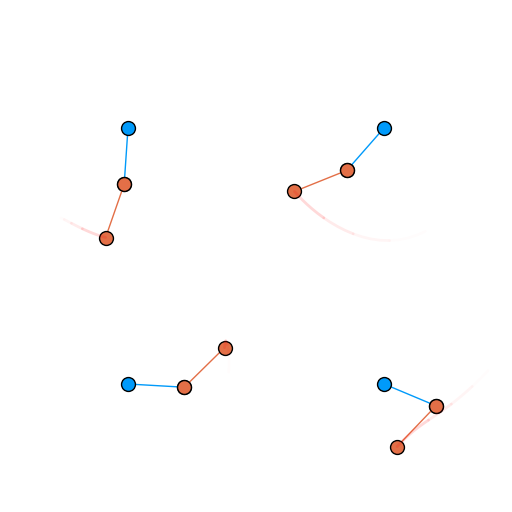
\includegraphics[width=\textwidth]{double_pendulum}}{imgs/double_pendulum.mp4}
		\end{center}
	\end{minipage}

	\vspace{-1cm}
\end{frame}

\begin{frame}[t, c]{Some examples}{Fluid dynamics}
  \begin{minipage}{.48\textwidth}
    \centering
    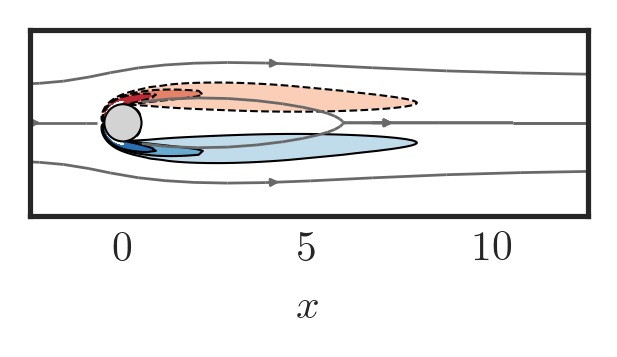
\includegraphics[width=\textwidth]{base_flow}

    \textbf{Below the critical Reynolds number}
  \end{minipage}%
  \hfill
  \begin{minipage}{.48\textwidth}
    \centering
    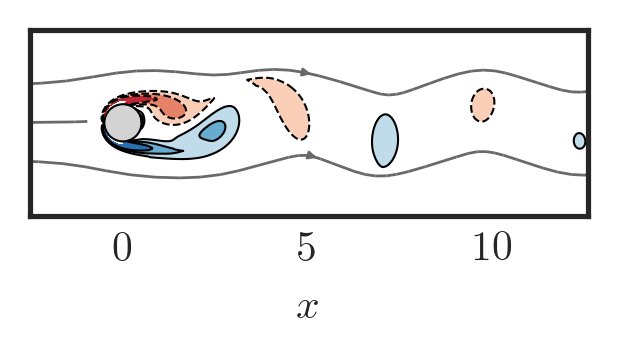
\includegraphics[width=\textwidth]{ground_truth_flow_field}

    \textbf{Above the critical Reynolds number}
  \end{minipage}

  \vspace{1cm}
\end{frame}

\begin{frame}[t, c]{Some examples}{Chemistry}
  \begin{minipage}{.38\textwidth}
    \centering
    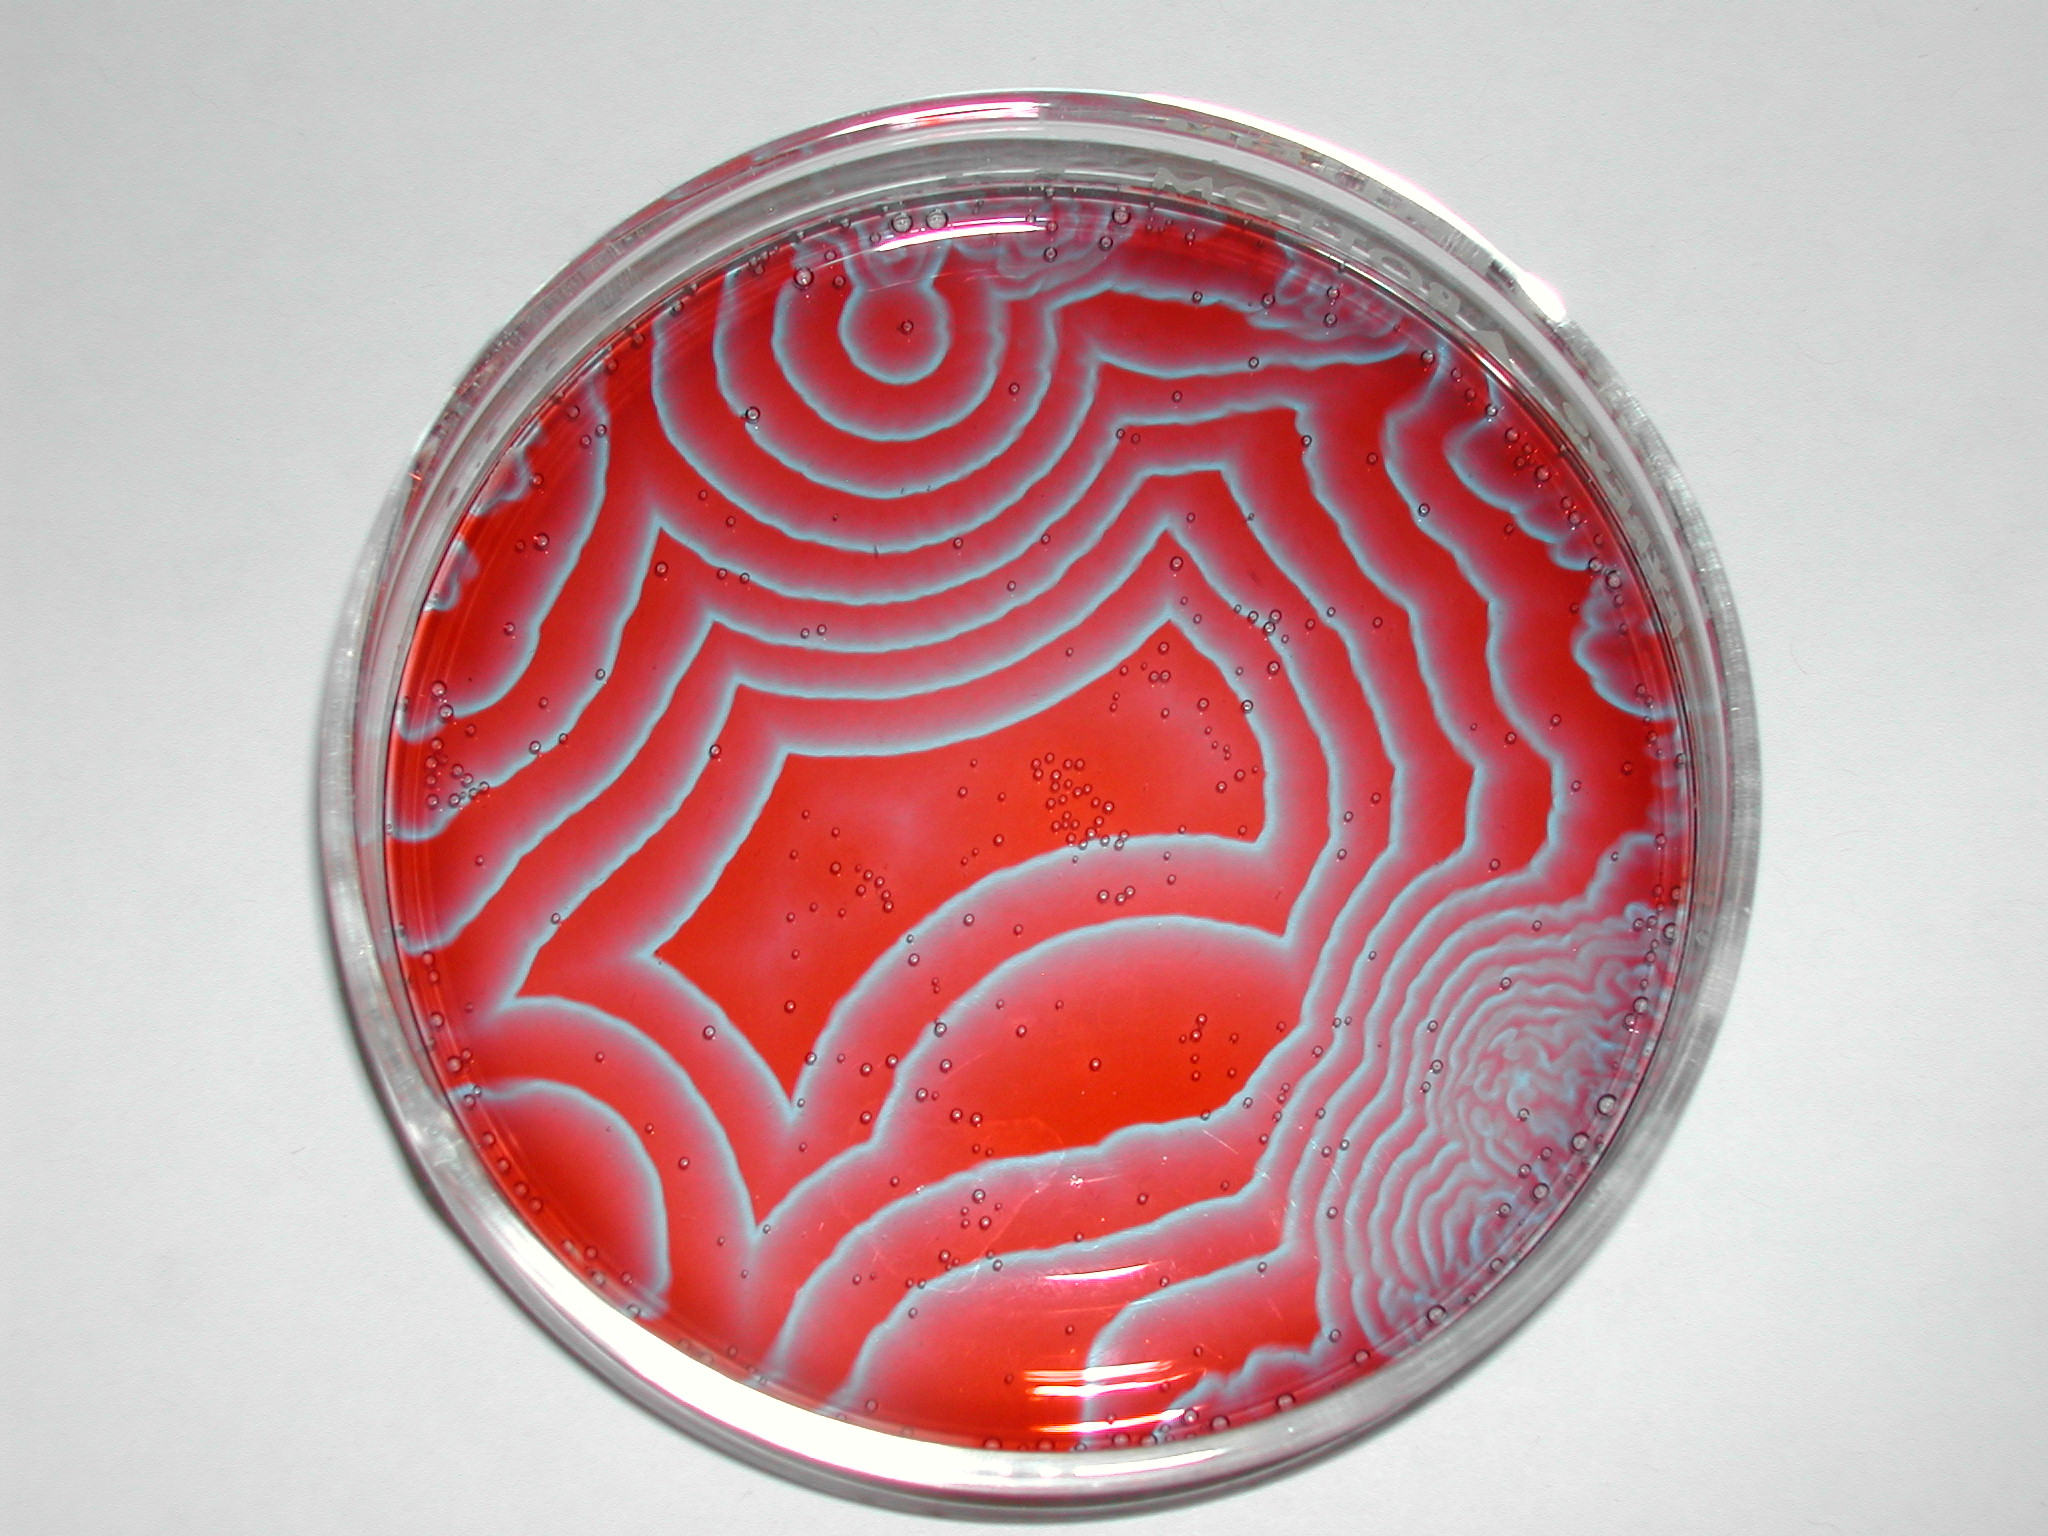
\includegraphics[width=\textwidth]{BZ_reaction}
  \end{minipage}%
  \hfill
  \begin{minipage}{.58\textwidth}
    \begin{itemize}
    \item Spatio-temporal system described by
      
      \[
      \dfrac{\partial \bm{q}_i}{\partial t} = \bm{D} \nabla^2 \bm{q}_i + \mathcal{R}(\bm{q}_i, \bm{q}_j)
      \]
      %
      where $\bm{D}$ describes the diffusion of each species and $\mathcal{R}(\bm{q}_i, \bm{q}_j)$ the inter-species reactions.

      \bigskip

    \item Can give rise to wonderful spatio-temporal patterns !
    \end{itemize}
  \end{minipage}

  \vspace{1cm}
\end{frame}

\begin{frame}[t, c]{Some examples}{Biology}
  \begin{minipage}{.38\textwidth}
    Synchronization occurs in numerous biological systems, e.g.
    \medskip
    \begin{itemize}
    \item Fireflies in South-East Asia,
    \item Pacemaker cells in the heart,
    \item Neurons during epilepsy,
    \item etc.
    \end{itemize}
  \end{minipage}%
  \hfill
  \begin{minipage}{.58\textwidth}
    \centering
    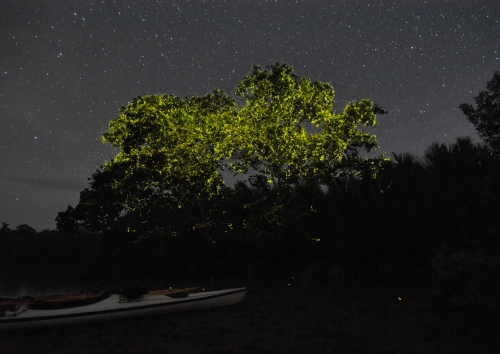
\includegraphics[width=.9\textwidth]{fireflies}
  \end{minipage}

  \vspace{1cm}
\end{frame}

\begin{frame}[t, c]{Some examples}{Epidemiology}
  \begin{minipage}{.58\textwidth}
    \centering
    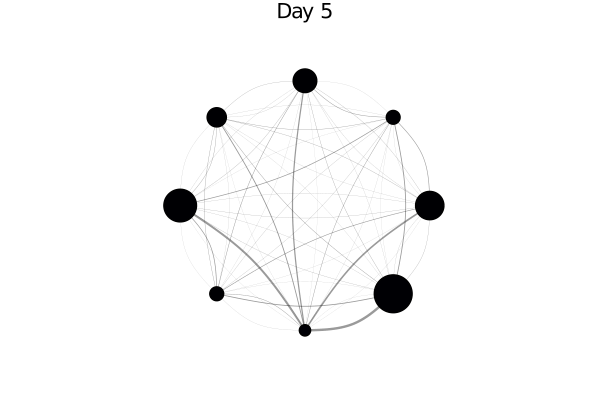
\includegraphics[width=\textwidth]{covid}

    \textbf{Combining epidemiology, dynamical \\ systems and graph theory}
  \end{minipage}%
  \hfill
  \begin{minipage}{.38\textwidth}
    \[
    \begin{aligned}
      \dfrac{\mathrm{d}s_i}{\mathrm{d}t} & = - \beta s_i i_i  \\
      \dfrac{\mathrm{d}i_i}{\mathrm{d}t} & = \beta s_i i_i - \gamma i_i + \sum_{i \neq j}^n \mathcal{R}_{ij}(\bm{x}_i, \bm{x}_j) \\
      \dfrac{\mathrm{d}r_i}{\mathrm{d}t} & = \gamma i_i
    \end{aligned}
    \]
  \end{minipage}

  \vspace{1cm}
\end{frame}

\begin{frame}[t, c]{}{}
  \begin{block}{\centering \textbf{How do we study them ?}}
    \bigskip

    \centering

    Find common patterns in the dynamics of seemingly different systems and distill them to their essence.

  \end{block}
\end{frame}

\begin{frame}[t, c]{How do we study them ?}{From a complex system to a simple model}
  \begin{minipage}{.38\textwidth}
    \centering
    \textbf{Mean-field model}
    %
    \[
    \begin{aligned}
      \dot{x} & = \sigma x - \omega y - xz \\
      \dot{y} & = \omega x + \sigma y - yz \\
      \dot{z} & = -\beta z + x^2 + y^2
    \end{aligned}
    \]
  \end{minipage}%
  \hfill
  \begin{minipage}{.58\textwidth}
    \centering
    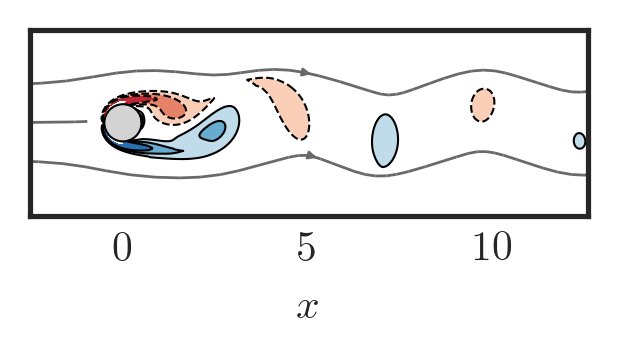
\includegraphics[width=\textwidth]{ground_truth_flow_field}
  \end{minipage}

  \vspace{1cm}
\end{frame}

\begin{frame}[t, c]{How do we study them ?}{From a complex system to a simple model}
  \begin{minipage}{.48\textwidth}
    \centering
    \textbf{Phase models}
    %
    \[
    \dot{\theta}_i = \omega_i + \dfrac{1}{N} \sum_{j \neq i}^N K_{ij} \sin(\theta_j - \theta_j)
    \]
  \end{minipage}%
  \hfill
  \begin{minipage}{.48\textwidth}
    \centering
    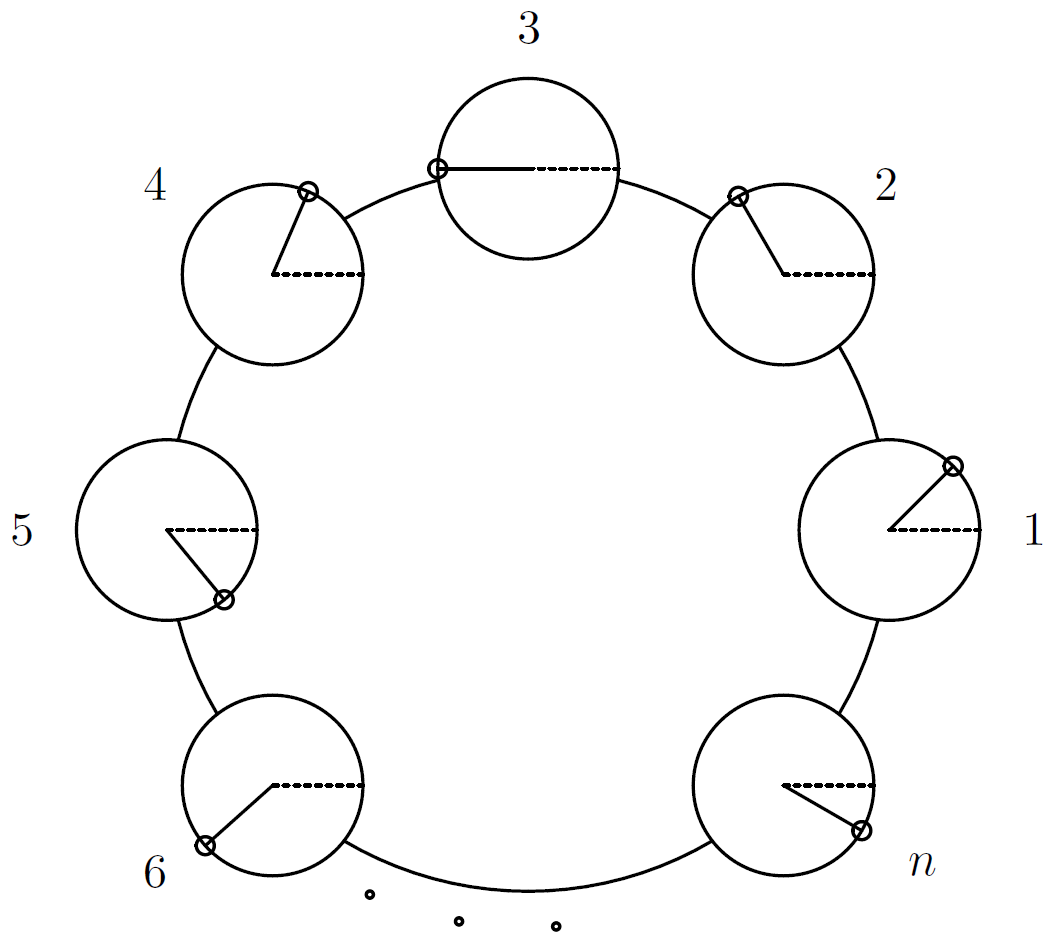
\includegraphics[width=\textwidth]{kuramoto}
  \end{minipage}

  \vspace{1cm}
\end{frame}

\begin{frame}[t, c]{How do we study them ?}{Looking for equilibrium solutions}
  \begin{minipage}{.38\textwidth}
    \centering
    \textbf{Fixed points}

    \medskip

    Given a nonlinear system $\dot{\bm{x}} = \bm{f}(\bm{x})$, find solutions to
    %
    \[
    \bm{f}(\bm{x}^*) = 0
    \]
  \end{minipage}%
  \hfill
  \begin{minipage}{.58\textwidth}
    \centering
    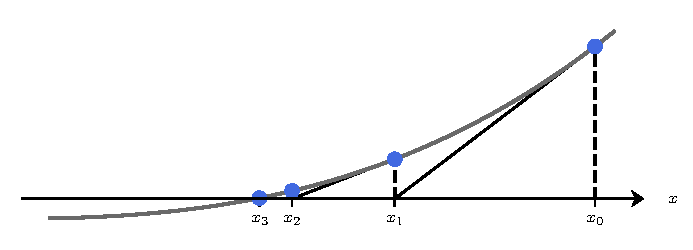
\includegraphics[width=\textwidth]{Newton_method}
  \end{minipage}

  \vspace{1cm}
\end{frame}

\begin{frame}[t, c]{How de we study them ?}{Perturbing equilibrium solutions}
  \begin{minipage}{.48\textwidth}
    \centering
    \textbf{Linear stability}
    %
    \[
    \begin{aligned}
      & \dot{\boldsymbol{\eta}} \simeq \bm{f}^{\prime}(\bm{x}^*) \boldsymbol{\eta} \\
      & \text{for } \| \boldsymbol{\eta} \| \ll 1
    \end{aligned}
    \]
  \end{minipage}%
  \hfill
  \begin{minipage}{.48\textwidth}
    \centering
    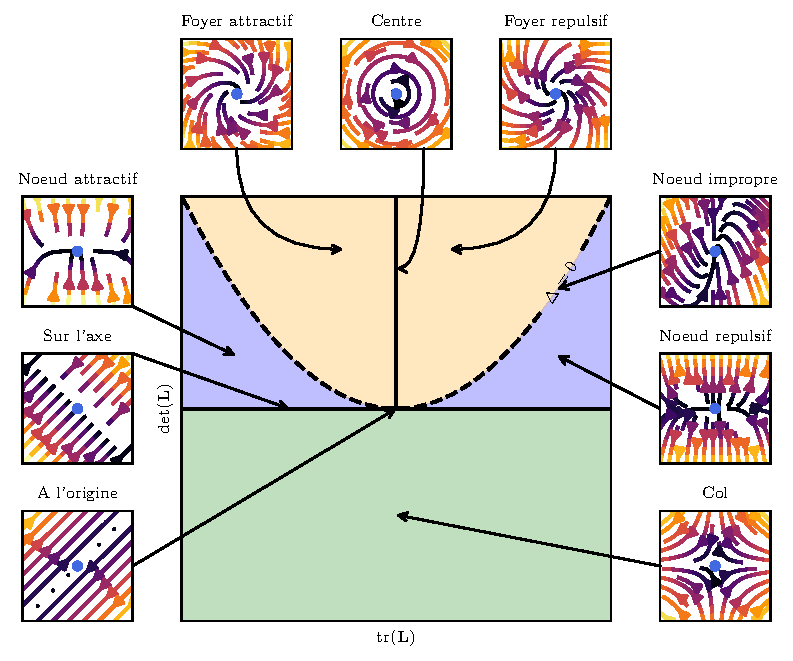
\includegraphics[width=\textwidth]{fixed_points_classification}
  \end{minipage}

  \vspace{1cm}
\end{frame}

\begin{frame}[t, c]{How de we study them ?}{Perturbing limit cycle solutions}
  \begin{minipage}{.48\textwidth}
    \centering
    \textbf{Poincaré-Lindsted}

    \medskip

    Rescale the solution and time according to
    %
    \[
    \begin{aligned}
      x(\tau) & = x_0(\tau) + \epsilon x_1(\tau) + \epsilon^2 x_2(\tau) + \cdots \\
      \tau & = \left(\omega_0 + \epsilon \omega_1 + \epsilon^2 \omega_2 + \cdots \right) t
    \end{aligned}
    \]
    %
    and solve a hierarchy of linear problems
    %
    \[
    \begin{aligned}
      & \mathcal{O}(0) : \quad \ddot{x}_0 - L(x_0) = 0\\
      & \mathcal{O}(1) : \quad \ddot{x}_1 - L(x_0, \omega_0)x_1 = F_1(x_0, \omega_0, \omega_1) \\
      & \mathcal{O}(2) : \quad \ddot{x}_2 - L(x_0, \omega_0)x_2 = F_2(x_0, x_1, \omega_0, \omega_1, \omega_2)
    \end{aligned}
    \]
  \end{minipage}%
  \hfill
  \begin{minipage}{.48\textwidth}
    \centering
    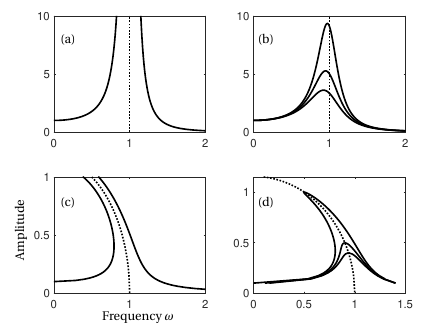
\includegraphics[width=\textwidth]{poincare_lindsted}
  \end{minipage}

  \vspace{1cm}
\end{frame}

\begin{frame}[t, c]{How do we study them ?}{Introduce new tools and new concepts}
  \begin{minipage}{.48\textwidth}
    \centering
    \textbf{Equation of a circle}
    %
    \[
    x^2 + y^2 = R^2
    \]
    \vspace{0.75cm}
  \end{minipage}%
  \hfill
  \begin{minipage}{.48\textwidth}
    
\begin{tikzpicture}
      \begin{polaraxis}[
          domain     = 0:180,
          samples    = 100,
          axis lines = none,
        ]
        \addplot[thick] {sin(x)};
      \end{polaraxis}
    \end{tikzpicture}
    \vspace{-1.5cm}
  \end{minipage}

\end{frame}


\begin{frame}[t, c]{How do we study them ?}{Introduce new tools and new concepts}
  \begin{minipage}{.48\textwidth}
    \centering
    \textbf{Quadratic map}
    %
    \[
    \begin{aligned}
      & x_{k+1} = x_k^2 + c, \\
      & x_0 = 0, \\
      & c \in \mathbb{C}
    \end{aligned}
    \]
  \end{minipage}%
  \hfill
  \begin{minipage}{.48\textwidth}
    \centering
    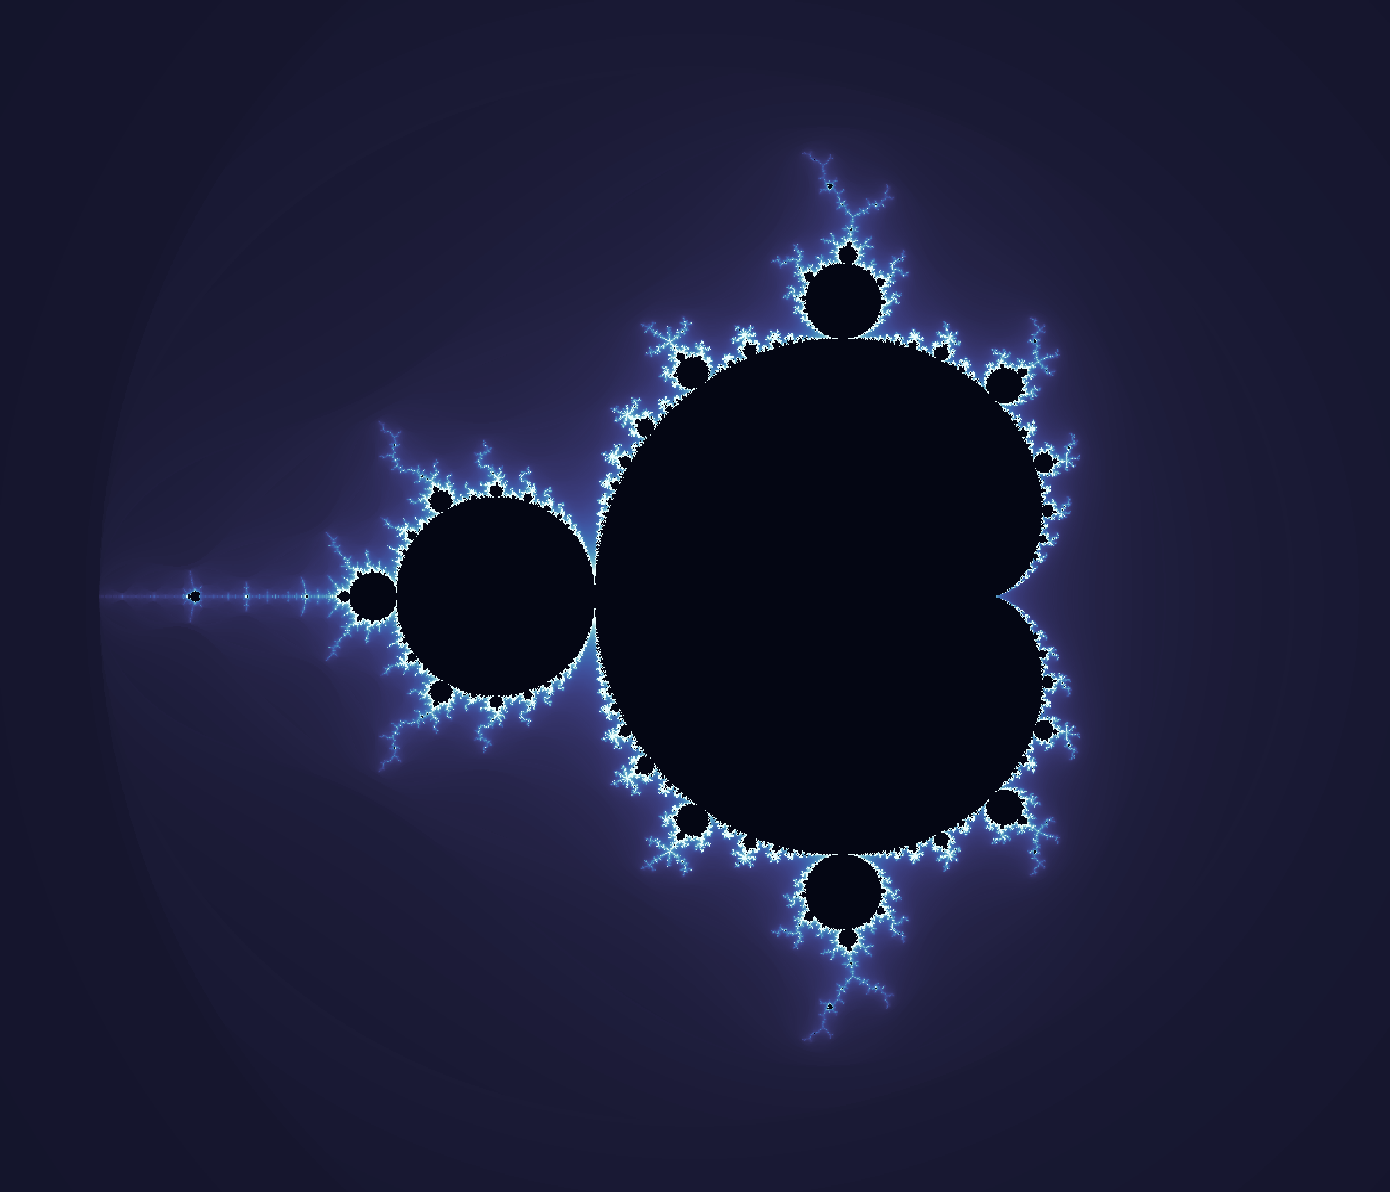
\includegraphics[width=\textwidth]{Mandelbrot_set}
  \end{minipage}

  \vspace{1cm}
\end{frame}

\begin{frame}[t, c]{Syllabus}{What you'll see in this course}
  \begin{minipage}{.68\textwidth}
    \begin{itemize}
    \item L2 : Fixed points and their linear stability
      \medskip
    \item L3 : Elements of bifurcation theory
      \medskip
    \item L4 : Limit cycles
      \medskip
    \item L5 : Synchronization and phase dynamics
      \medskip
    \item L6-L9 : Chaos and strange attractors
      \medskip
    \item L10 : Cellular automata
      \medskip
    \item L11-L15 : Data-driven methods for dynamical systems
    \end{itemize}
  \end{minipage}%
  \hfill
  \begin{minipage}{.28\textwidth}
    \centering
    
\includegraphics[width=\textwidth]{Gears}
  \end{minipage}

  \vspace{1cm}
\end{frame}

\begin{frame}[t, c]{Syllabus}{What you'll need}
  \begin{minipage}{.58\textwidth}
    This is an 'informal' course on dynamical systems.
    We'll focus on intuition and liberal use of computers rather than proper mathemetical proofs.

    \bigskip

    We'll still need a bit of maths though :
    \begin{itemize}
    \item \textbf{Linear algebra} : eigenvalues and eigenvectors
    \item \textbf{Calculus} : Ordinary differential equations, Power series, Fourier series, Taylor series
    \item \textbf{Numerical analysis} : Temporal integration, root finding
    \end{itemize}
  \end{minipage}%
  \hfill
  \begin{minipage}{.38\textwidth}
    \centering
    
\includegraphics[width=\textwidth]{still_waiting}
  \end{minipage}

  \vspace{1cm}
\end{frame}

\end{document}
